%% Fail-Closed Provider Execution for Governed AI Agent Runtimes
%% IEEEtran conference format. Derived from the \Argorix preprint; no new
%% experiments, metrics, citations, or deployment claims are introduced.
\documentclass[conference]{IEEEtran}
\IEEEoverridecommandlockouts

\usepackage[T1]{fontenc}
\usepackage[utf8]{inputenc}
\usepackage{cite}
\usepackage{amsmath,amssymb}
\usepackage{graphicx}
\usepackage{booktabs}
\usepackage{array}
\usepackage{xcolor}
\usepackage{listings}
\usepackage{tikz}
\usetikzlibrary{arrows.meta,positioning,fit,backgrounds,shapes.geometric,calc}
\usepackage{url}
\usepackage{xspace}
\usepackage[hidelinks]{hyperref}

% Compact monospace helper for inline identifiers/fields.
\newcommand{\code}[1]{\texttt{\small #1}}
% Ragged-right paragraph column for tables (avoids overfull monospace cells).
\newcolumntype{L}[1]{>{\raggedright\arraybackslash}p{#1}}

% \Argorix brand wordmark: per-character gradient across the brand palette
% (reused from the original \Argorix preprint preamble).
\definecolor{argViolet}{HTML}{7C3AED}
\definecolor{argIndigo}{HTML}{5B3DF5}
\definecolor{argElectric}{HTML}{2F6BFF}
\definecolor{argCyan}{HTML}{2BC4F4}
\definecolor{argCyanBright}{HTML}{5CD6FF}
\newcommand{\Argorix}{%
\textcolor{argViolet}{A}\textcolor{argViolet}{r}\textcolor{argIndigo}{g}\textcolor{argIndigo}{o}\textcolor{argElectric}{r}\textcolor{argElectric}{i}\textcolor{argElectric}{x}\textcolor{argCyan}{L}\textcolor{argCyan}{a}\textcolor{argCyanBright}{n}\textcolor{argCyanBright}{g}\xspace}

% Listing style for the planning algorithm.
\lstset{basicstyle=\ttfamily\scriptsize,breaklines=true,frame=single,
  columns=fullflexible,keepspaces=true,xleftmargin=0.5em}

% Shared TikZ styles for figure stubs.
\tikzset{
  ebox/.style={draw,rounded corners=2pt,align=center,inner sep=3pt,
    font=\scriptsize,minimum height=6mm},
  eimpl/.style={ebox,fill=black!4},
  eprop/.style={ebox,draw,dashed,fill=white},
  edeny/.style={ebox,fill=argViolet!10,draw=argViolet!60},
  eflow/.style={-{Latex[length=2mm]},thin},
  edash/.style={-{Latex[length=2mm]},thin,dashed},
}

\begin{document}

\title{Fail-Closed Provider Execution\\for Governed AI Agent Runtimes}

\author{
\IEEEauthorblockN{Gustavo Venegas\IEEEauthorrefmark{1},
Edison Vazquez\IEEEauthorrefmark{1},
Danilo Naranjo\IEEEauthorrefmark{2},
Benjamin Gonzalez\IEEEauthorrefmark{1}}
\IEEEauthorblockA{\IEEEauthorrefmark{1}Chilean Chamber of Artificial Intelligence\quad
\IEEEauthorrefmark{2}Ocular\\
\texttt{\footnotesize gustavo@gobiernoia.cl,\ edison@jhedai.com,\ dan@ocularsolution.com,\ ben@nirvana-ai.com}}
}

\maketitle

\begin{abstract}
Governed AI agent runtimes interleave model calls, tool decisions, and provider
operations, and a single request that crosses the provider boundary can trigger external
calls, data movement, network access, or credential use. A recurring hazard is that
declared provider metadata is treated as executable authority: a contract that names an
external provider is allowed to select it. We present \Argorix's \emph{fail-closed
provider boundary}, which separates declarative provider contracts from executable
provider adapters and applies capability, policy, and runtime-profile checks before any
provider operation is planned. Only providers explicitly enrolled in an executable
registry are callable; a named contract is metadata, not authority. We give a lightweight
formal model of the planning rule---$\mathrm{Plan}\Rightarrow\mathrm{MayExecute}$, with
$\mathrm{Declared}\nRightarrow\mathrm{Executable}$---and an authorization algorithm in
which any unknown reference, denied capability, failed policy, or non-executable provider
terminates in a recorded denial or review state rather than falling through to execution.
On the existing \Argorix corpus of 33 request directories (27 complete, 6 source-only),
the evaluated profile is simulated-only: every complete trace records an external-provider
execution blocked event, network denied, and secrets/key-material denied. We hold a strict
boundary: VM-level denial does not prove operating-system sandboxing, container isolation,
host network containment, secret-store isolation, adapter correctness, absence of side
effects, or production isolation.
\end{abstract}

\begin{IEEEkeywords}
AI agents, governed runtime, fail-closed execution, provider boundary, runtime security,
policy enforcement, capability checks, agent governance, negative controls.
\end{IEEEkeywords}

\section{Introduction}\label{sec:intro}
The provider boundary is the most consequential decision point in a governed AI agent
runtime. Everything upstream of it---prompt parsing, planning, tool selection---is
internal deliberation; the moment an agent \emph{executes} a provider operation, the
runtime can issue an external call, move data off the host, open a network connection, or
read credential material. If that boundary is permissive, the rest of the governance stack
is decoration: a system that carefully records policy decisions but then lets any declared
provider run has recorded nothing that constrains behavior.

The specific failure mode we target is the conflation of \emph{declaration} with
\emph{authority}. Agent programs, prompts, and configuration routinely \emph{name}
providers---an OpenAI provider, a search tool, a remote model. A naive runtime treats the
appearance of a provider name as permission to call it, so that adding a line of metadata,
or coaxing the model into emitting one, selects an external execution path. Governed
runtimes must not allow prompts, source-level declarations, or contract metadata to
\emph{become} executable authority. A declared provider contract should describe an
intended boundary; it should not, by itself, make a provider callable.

\Argorix \cite{venegas2026argorixlang,argorixlang2026} enforces this separation at the
virtual-machine level. Its provider boundary maintains two distinct registries: a set of
\emph{declarative provider contracts} (capabilities, limits, intended operations) and a
set of \emph{executable provider adapters} (callable implementations). A contract's
presence does not enroll its provider for execution. Before any operation is planned, the
runtime evaluates capability constraints, policy permission, and a runtime profile, and
consults the executable registry. The governing rule is \emph{fail-closed}: when a
reference is unknown, a capability is incompatible, a policy denies or requires review, or
a provider is not executable, the request path terminates in an auditable denial or review
state rather than falling through to a provider call.

We are deliberate about what this does and does not establish. Fail-closed here is a
control-flow property of the implemented VM/application path: missing authorization does
not reach execution. It is \emph{not} a proof of operating-system sandboxing, container
isolation, host-level network containment, secret-store isolation, live-provider safety,
adapter correctness, or absence of side effects outside instrumentation. We keep that
boundary explicit throughout.

\noindent\textbf{Contributions.}
\begin{enumerate}
\item A fail-closed execution model for governed AI agent runtimes, in which absence of
authorization yields denial or review rather than fallthrough execution.
\item A provider-boundary design that separates declarative contracts from executable
adapters, with an executable registry as the sole source of callable providers.
\item A lightweight formal model of provider-execution authorization, stated as an
interpretation of the implemented planning rule rather than a verification proof.
\item An observational evaluation on the existing \Argorix corpus showing blocked external
execution, network denial, and secret/key-material denial.
\item A strict claim-boundary analysis distinguishing VM-level denial from production
isolation.
\end{enumerate}

A scope note distinguishing this paper from the companion Agent Passport and
EvidenceBundle papers is given in Section~\ref{sec:diff}.

\section{Background and Motivation}\label{sec:background}
A governed agent runtime is a composition of model calls, tools, provider adapters,
policies, and evidence. These layers fail differently, and the provider layer fails
hardest, because it is the only one whose outputs leave the runtime. A wrong tool plan can
be re-planned; an executed external provider call cannot be un-sent.

It helps to separate concepts that informal usage collapses. A \emph{provider declaration}
is the appearance of a provider name in a program or request. A \emph{provider contract} is
structured metadata describing a provider's capabilities, operation limits, and intended
boundary. An \emph{executable adapter} is a runtime-callable implementation. A
\emph{capability permission} is an agent's right to perform an operation class. A
\emph{runtime profile} is the per-execution policy on network, secrets, key material,
tools, and external execution. A \emph{policy approval} is a decision over a specific
operation. And \emph{actual external execution} is the act of invoking a live provider.
These are not synonyms, and a safe runtime requires \emph{all} of the gating conditions to
hold before reaching the last one.

\emph{Fail-open} behavior---defaulting to execution when a check is missing,
unrecognized, or errors---is dangerous precisely because the dangerous path is the default.
A misconfigured registry entry, an unhandled lookup miss, or an ambiguous policy result
becomes an external call. Fail-closed inverts the default: the absence of a positive
authorization is itself a denial. This makes \emph{negative controls}---recorded events
showing that an operation was blocked, that network was denied, that secrets were
withheld---first-class evidence. A negative control is positive evidence of denial
behavior. It is not, and we do not read it as, proof of host-level containment.

\section{Provider Boundary Model}\label{sec:model}
We define the boundary in terms of six elements; Table~\ref{tab:concepts} summarizes their
implemented role and what each does \emph{not} claim.

\emph{(1) Declarative provider contract.} A contract names a provider and states its
capabilities, operation limits, and intended boundary. It is metadata only. A contract is
inert with respect to execution: it cannot, by itself, cause a provider call. In the
evaluated chatbot artifacts, an \code{OpenAIProvider} contract and an \code{OpenAISandbox}
descriptor are present as declarations.

\emph{(2) Executable provider adapter.} An adapter is a runtime-callable implementation.
It is reachable only if explicitly enrolled in the executable provider registry, and even
then only after capability, policy, and runtime-profile checks succeed.

\emph{(3) Executable provider registry.} The registry is the sole source of callable
providers. A provider named in a contract is not callable unless it also appears in the
registry. In the observed configuration the only executable provider is \code{simulated};
external providers named by declarations remain non-executable.

\emph{(4) Runtime profile.} The profile denies, for the demonstrated path, network access,
plaintext secrets, key material, tools, agent execution, and external execution, and
requires audit, evidence, security reports, and sandbox metadata. It is consulted before
planning.

\emph{(5) Provider boundary events.} The runtime emits auditable events at the boundary,
including an external-provider execution blocked event, a runtime network denied event, and
a runtime secrets denied event, each recorded in the trace.

\emph{(6) The key distinction.} The model's load-bearing statement is that declaration does
not imply executability:
\[
\mathrm{Declared}(p)\ \nRightarrow\ \mathrm{Executable}(p).
\]
A contract may name an external provider; a contract does not make a provider executable.

\begin{table}[t]
\centering
\caption{Provider boundary concepts.}
\label{tab:concepts}
\renewcommand{\arraystretch}{1.25}
\scriptsize
\setlength{\tabcolsep}{3pt}
\begin{tabular}{@{}L{0.17\columnwidth}L{0.24\columnwidth}L{0.24\columnwidth}L{0.21\columnwidth}@{}}
\toprule
\textbf{Concept} & \textbf{Meaning} & \textbf{Implemented role} & \textbf{Not claimed} \\
\midrule
Declarative contract & Provider name, capabilities, limits & Inert metadata; intended boundary & Executable authority \\
Executable adapter & Callable implementation & Reachable only if registered & Adapter correctness/safety \\
Executable registry & Set of callable providers & Sole source of execution; \code{simulated} only & Live external providers \\
Runtime profile & Per-run denials & Denies net/secrets/keys/ext.\ exec & Host-level containment \\
Capability check & Agent's right to an op & Gate before planning & Identity verification \\
Boundary event & Recorded denial/block & Auditable negative control & OS sandbox proof \\
\bottomrule
\end{tabular}
\end{table}

\begin{figure}[t]
\centering
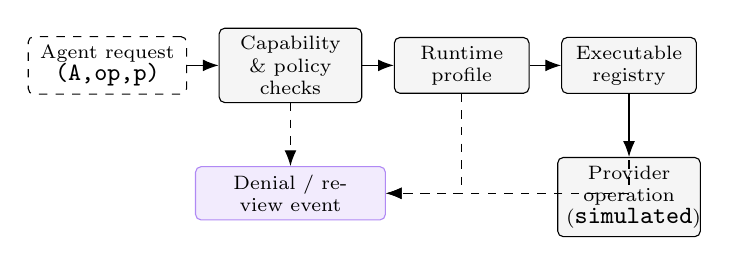
\begin{tikzpicture}[font=\scriptsize,node distance=4mm]
\node[eprop,text width=18mm] (req) {Agent request \code{(A,op,p)}};
\node[eimpl,right=of req,text width=16mm] (cap) {Capability \& policy checks};
\node[eimpl,right=of cap,text width=15mm] (rp) {Runtime profile};
\node[eimpl,right=of rp,text width=15mm] (reg) {Executable registry};
\node[eimpl,below=8mm of reg,text width=16mm] (exec) {Provider operation (\code{simulated})};
\node[edeny,below=8mm of cap,text width=22mm] (deny) {Denial / review event};
\draw[eflow] (req)--(cap); \draw[eflow] (cap)--(rp); \draw[eflow] (rp)--(reg);
\draw[eflow] (reg)--(exec);
\draw[edash] (cap) -- (deny);
\draw[edash] (rp) |- (deny);
\draw[edash] (reg) |- (deny);
\end{tikzpicture}
\caption{Provider boundary architecture. An agent request passes capability/policy checks,
the runtime profile, and the executable registry before any provider operation is planned;
any failing gate diverts to a recorded denial or review event.}
\label{fig:arch}
\end{figure}

\begin{figure}[t]
\centering
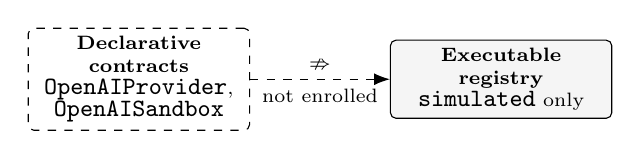
\begin{tikzpicture}[font=\scriptsize]
\node[eprop,text width=26mm] (c) at (0,0) {\textbf{Declarative contracts}\\\code{OpenAIProvider},\\\code{OpenAISandbox}};
\node[eimpl,text width=26mm] (e) at (4.6,0) {\textbf{Executable registry}\\\code{simulated} only};
\draw[edash] (c) -- node[midway,above,font=\scriptsize]{$\nRightarrow$} node[midway,below,font=\scriptsize]{not enrolled} (e);
\end{tikzpicture}
\caption{Declarative vs.\ executable split. Contract metadata (left) names providers but
does not enroll them; only the executable registry (right) yields callable providers. A
contract does not imply an executable adapter.}
\label{fig:split}
\end{figure}

\section{Formal Model}\label{sec:formal}
We give a lightweight formalization. It is a precise \emph{runtime interpretation} of the
implemented fail-closed boundary, not a full formal-verification proof.

\noindent\textbf{Definitions.} Let $A$ be the requesting agent, $op$ the requested
operation, and $p$ the target provider. Let $C$ be the set of declared provider contracts
and $E$ the executable provider registry. Define predicates: $\mathrm{Declared}(p)
:\Leftrightarrow p\in C$; $\mathrm{Executable}(p):\Leftrightarrow p\in E$;
$\mathrm{Cap}(A,op)$, agent $A$ holds the capability for $op$; $\mathrm{PolicyPermit}(A,op,p)$,
the policy permits the operation; $\mathrm{RuntimePermit}(op,p)$, the runtime profile permits
it. Let $\mathrm{Plan}(A,op,p)$ mean the VM may plan execution of $op$ on $p$, and
$\mathrm{Deny}(A,op,p)$ mean the VM terminates the request path with a denial or review
event.

\noindent\textbf{Authorization predicate.}
\begin{align*}
\mathrm{MayExecute}(A,op,p) :=\ &
\mathrm{Executable}(p) \\
\wedge\ & \mathrm{Cap}(A,op) \\
\wedge\ & \mathrm{PolicyPermit}(A,op,p) \\
\wedge\ & \mathrm{RuntimePermit}(op,p)
\end{align*}

\noindent\textbf{Fail-closed planning rule.} Planning requires authorization, and its
contrapositive is denial:
\[
\mathrm{Plan}(A,op,p)\ \Rightarrow\ \mathrm{MayExecute}(A,op,p),
\]
\[
\neg\mathrm{MayExecute}(A,op,p)\ \Rightarrow\ \mathrm{Deny}(A,op,p).
\]

\noindent\textbf{Declaration is not executability.} The boundary statement and its
consequence:
\[
\mathrm{Declared}(p)\ \nRightarrow\ \mathrm{Executable}(p),
\]
\[
\mathrm{Declared}(p)\wedge\neg\mathrm{Executable}(p)\ \Rightarrow\ \neg\mathrm{MayExecute}(A,op,p).
\]
In particular, an external provider that is declared but not enrolled is blocked:
\begin{multline*}
\mathrm{ExternalProviderDeclared}(p)\wedge p\notin E\\
\Rightarrow\ \textsf{ExternalProviderExecutionBlocked}.
\end{multline*}

\noindent\textbf{Reading.} The conjunction in $\mathrm{MayExecute}$ is the formal content
of fail-closed: every conjunct must hold to plan, so the failure (or absence) of any one
forces $\mathrm{Deny}$. We do not present this as proof of authenticity, isolation, or
external truth; it is a statement about the implemented control flow, in which
non-authorization cannot reach a provider call. Table~\ref{tab:predicates} restates the
predicates.

\begin{table}[t]
\centering
\caption{Fail-closed authorization predicates.}
\label{tab:predicates}
\renewcommand{\arraystretch}{1.3}
\scriptsize
\setlength{\tabcolsep}{3pt}
\begin{tabular}{@{}L{0.26\columnwidth}L{0.32\columnwidth}L{0.30\columnwidth}@{}}
\toprule
\textbf{Predicate} & \textbf{Definition} & \textbf{Interpretation} \\
\midrule
$\mathrm{Executable}(p)$ & $p\in E$ & Provider enrolled as callable \\
$\mathrm{Declared}(p)$ & $p\in C$ & Provider named by a contract \\
$\mathrm{MayExecute}$ & Exec $\wedge$ Cap $\wedge$ Policy $\wedge$ Runtime & All gates hold \\
$\mathrm{Plan}\Rightarrow\mathrm{MayExecute}$ & planning needs authorization & Fail-closed rule \\
$\neg\mathrm{MayExecute}\Rightarrow\mathrm{Deny}$ & contrapositive & No fallthrough \\
$\mathrm{Declared}\nRightarrow\mathrm{Executable}$ & contract $\neq$ adapter & Boundary statement \\
\bottomrule
\end{tabular}
\end{table}

\section{Runtime Execution Sequence}\label{sec:sequence}
The runtime evaluates a validated program rather than accepting unrestricted provider
calls. The path proceeds: (1) load validated bytecode; (2) resolve the requesting agent
and handler; (3) resolve target provider metadata; (4) evaluate capability constraints;
(5) evaluate policy constraints; (6) consult the runtime profile; (7) consult the
executable provider registry; (8) plan the operation only if all checks pass; (9)
otherwise emit a denial or review event and do not execute; (10) record trace, security
report, and evidence artifacts. Runtime state is retained in an outcome object even when
execution fails, so a report can describe the denial without converting it into success.
Algorithm~\ref{alg:plan} states the planning decision; Figure~\ref{fig:fsm} shows the
state machine.

\begin{figure}[t]
\lstset{caption={},label={}}
\begin{lstlisting}
Algorithm 1: Fail-Closed Provider Planning
Input : agent A, operation op, provider p,
        registry E, policy state Pi,
        runtime profile R
Output: plan or deny

 1. Resolve A, op, p.
 2. if A unknown or op unknown: deny.
 3. if p not in E:
       emit ExternalProviderExecutionBlocked; deny.
 4. if not Cap(A, op): deny.
 5. if not PolicyPermit(A, op, p):
       require review or deny.
 6. if not RuntimePermit(op, p):
       emit relevant denial event; deny.
 7. plan op only if (2)-(6) all pass.
 8. record decision in trace + security report.
\end{lstlisting}
\caption{Fail-closed provider planning. Each gate can only deny or pass; planning is
reached only when every gate passes.}
\label{alg:plan}
\end{figure}

\begin{figure}[t]
\centering
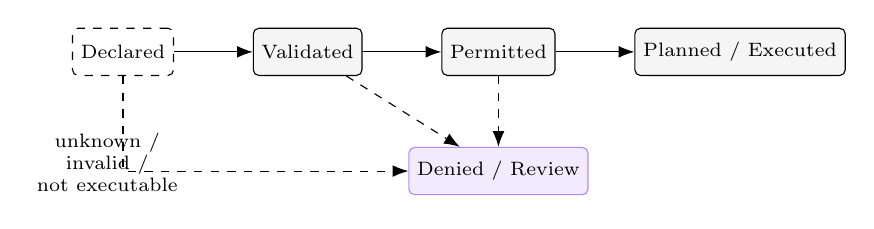
\begin{tikzpicture}[font=\scriptsize,node distance=7mm and 10mm]
\node[eprop] (decl) {Declared};
\node[eimpl,right=of decl] (val) {Validated};
\node[eimpl,right=of val] (perm) {Permitted};
\node[eimpl,right=of perm] (plan) {Planned / Executed};
\node[edeny,below=9mm of perm] (deny) {Denied / Review};
\draw[eflow] (decl)--(val); \draw[eflow] (val)--(perm); \draw[eflow] (perm)--(plan);
\draw[edash] (decl) |- (deny) node[pos=0.25,left,font=\scriptsize]{};
\draw[edash] (val) -- (deny);
\draw[edash] (perm) -- (deny);
\node[font=\scriptsize,align=center] at (-0.2,-1.4) {unknown /\\ invalid /\\ not executable};
\end{tikzpicture}
\caption{Fail-closed state machine. A request advances Declared $\to$ Validated $\to$
Permitted $\to$ Planned/Executed only while every gate passes; any unknown, invalid,
non-executable, or denied condition diverts to a recorded Denied/Review state.}
\label{fig:fsm}
\end{figure}

\section{Negative Controls}\label{sec:negative}
The evaluated profile exhibits a set of \emph{negative controls}: recorded outcomes in
which an operation was withheld. These include external-provider execution blocked, network
denied, secrets denied, key material denied, simulated-only provider execution, and
tools/agent-execution disabled for the demonstrated path; policy may additionally place a
request in a review-required state.

We read negative controls as \emph{positive evidence of denial behavior}: the runtime did
not merely fail to call an external provider, it recorded that it blocked one, denied
network, and withheld secrets. That recorded refusal is auditable and reproducible from the
artifacts. What a negative control is \emph{not} is proof of operating-system-level
containment: the runtime did not contact the provider, but this study does not instrument
the host to prove that no other process path could. The negative control evidence is
summarized in Figure~\ref{fig:neg} and quantified in Section~\ref{sec:eval}.

\begin{figure}[t]
\centering
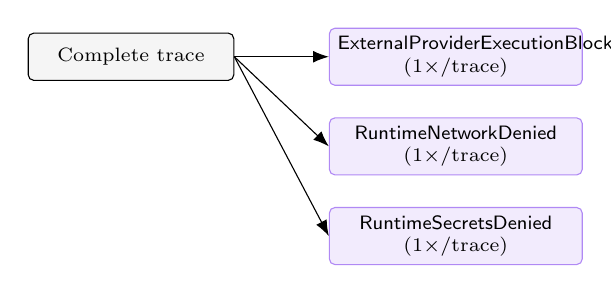
\begin{tikzpicture}[font=\scriptsize,node distance=4mm]
\node[eimpl,text width=24mm] (tr) {Complete trace};
\node[edeny,right=12mm of tr,text width=30mm] (e1) {\textsf{ExternalProviderExecutionBlocked} (1$\times$/trace)};
\node[edeny,below=of e1,text width=30mm] (e2) {\textsf{RuntimeNetworkDenied} (1$\times$/trace)};
\node[edeny,below=of e2,text width=30mm] (e3) {\textsf{RuntimeSecretsDenied} (1$\times$/trace)};
\draw[eflow] (tr.east) -- (e1.west);
\draw[eflow] (tr.east) -- (e2.west);
\draw[eflow] (tr.east) -- (e3.west);
\end{tikzpicture}
\caption{Negative control evidence. Each complete trace records the boundary denial events
as auditable negative controls; they are evidence of denial behavior, not OS-level
containment.}
\label{fig:neg}
\end{figure}

\section{Observational Evaluation}\label{sec:eval}
We reuse the existing \Argorix runtime corpus \cite{venegas2026argorixlang} and add no new
experiment, benchmark, or deployment.

\subsection{Corpus}
Of \textbf{33} request directories, \textbf{27} are \emph{complete} and \textbf{6} are
\emph{source-only} and not assessable for trace, security, or evidence fields. All 27
complete sessions report execution status \emph{completed}, and all 27 complete evidence
bundles pass offline verification (27/27). The corpus contains \textbf{7{,}155} counted
ledger events and \textbf{1{,}188} detailed policy violations across the complete sessions.

\subsection{Provider boundary and negative controls}
The evaluated runtime profile is \emph{simulated-only}: the executable provider registry
contains only the \code{simulated} provider, while declarative contracts name external
providers that remain non-executable. Each complete trace records one
\textsf{ExternalProviderExecutionBlocked} event, one \textsf{RuntimeNetworkDenied}, and one
\textsf{RuntimeSecretsDenied}; key material is likewise denied. The four observed runtime
controls are application-level behaviors (Table~\ref{tab:controls}).

\subsection{Policy results}
The detailed policy objects report \code{policy\_passed=false} and
\code{review\_required=true} for the complete sessions. A favorable coarse status field
does not override these detailed results: an explicit failure or required review prevents
an aggregate pass.

\subsection{Interpretation}
The observed profile demonstrates VM-level denial and bounded provider planning: external
execution is blocked, network and secrets are denied, and only a simulated provider is
callable. It does \emph{not} demonstrate live-provider safety, OS-level sandboxing, or
production isolation. Source-only directories remain \emph{unavailable}, never successful
executions; a missing artifact is an explicit incomplete observation, not a pass. The
repeated structure supports pipeline reproducibility but limits any claim of behavioral
diversity.

\begin{table}[t]
\centering
\caption{Observed runtime controls.}
\label{tab:controls}
\renewcommand{\arraystretch}{1.25}
\scriptsize
\setlength{\tabcolsep}{3pt}
\begin{tabular}{@{}L{0.30\columnwidth}L{0.26\columnwidth}L{0.30\columnwidth}@{}}
\toprule
\textbf{Control / event} & \textbf{Observed value} & \textbf{Interpretation} \\
\midrule
Provider execution & \code{simulated} only & Bounded executable registry \\
External execution & Blocked (1$\times$/trace) & Denial recorded, not isolation \\
Network access & Denied (1$\times$/trace) & VM-level egress refusal \\
Secrets / key material & Denied (1$\times$/trace) & No plaintext secret/key use \\
Complete directories & 27 / 33 & Assessable sessions \\
Source-only directories & 6 / 33 & Unavailable, not passes \\
Bundles verified offline & 27 / 27 & Internal consistency only \\
Ledger events & 7{,}155 & Structured event emission \\
Policy violations & 1{,}188 & Negatives preserved \\
Detailed policy result & passed=false, review=true & Review state preserved \\
\bottomrule
\end{tabular}
\end{table}

\section{Security Analysis}\label{sec:security}
We analyze threats as attack paths across trust boundaries, not as proof that a named
control defeats every adversary. Table~\ref{tab:threats} states each bounded mitigation
alongside its remaining gap.

\noindent\textbf{Threats.} A prompt- or source-level attempt to \emph{select} an external
provider; confusing a declarative contract with an executable adapter; capability
escalation; policy bypass; network egress through a live adapter; secret or key leakage; a
malicious executable adapter once registered; registry misconfiguration; runtime-status
confusion (reading a coarse pass over a detailed failure); host-level side effects outside
instrumentation; and consumer overinterpretation of VM denial as production security.

\noindent\textbf{Bounded mitigations.} The split between declarative and executable
registries prevents a contract from becoming callable merely by being named. The
executable registry is the sole execution source; capability and policy checks gate
planning; the runtime profile denies network, secrets, key material, and external
execution; the fail-closed rule forces denial on any missing authorization; and boundary
denials are recorded as auditable events preserved in evidence artifacts.

\noindent\textbf{Remaining risks.} A malicious or defective adapter, \emph{once enrolled},
is within the trust boundary and is not evaluated here. OS-level leakage, host network
misconfiguration, and secret-store exposure are outside the instrumented path. Evidence
bundles are unsigned, so an adversary controlling artifacts and bundle together can produce
a self-consistent replacement. There is no controlled adversarial test and no proof that
all side effects are blocked. The strongest supported statement is conditional: within the
observed runtime path, provider selection is mediated by capability, policy, and an
executable-provider allowlist; denials are recorded; and complete artifacts are
offline-consistent. Security outside that path remains unmeasured.

\begin{table}[t]
\centering
\caption{Threats and bounded mitigations.}
\label{tab:threats}
\renewcommand{\arraystretch}{1.25}
\scriptsize
\setlength{\tabcolsep}{3pt}
\begin{tabular}{@{}L{0.27\columnwidth}L{0.30\columnwidth}L{0.29\columnwidth}@{}}
\toprule
\textbf{Threat} & \textbf{Bounded mitigation} & \textbf{Remaining gap} \\
\midrule
Select external provider via metadata & Declarative/executable split; registry is sole source & Adapter behavior once enrolled \\
Capability escalation & Capability check before planning & No identity verification \\
Policy bypass & Policy permit / review before planning & Decision not canonicalized \\
Network egress & Runtime profile denies network & No host egress proof \\
Secret / key leakage & Secret and key-material denial & No secret-store isolation \\
Malicious adapter & Registry enrollment required & Registered adapter untested \\
Status confusion & Detail dominates coarse status & Schema-level precedence pending \\
Overinterpretation & Explicit claim boundary & Consumer discipline required \\
\bottomrule
\end{tabular}
\end{table}

\begin{table}[t]
\centering
\caption{Declared vs.\ executable provider distinction.}
\label{tab:declexec}
\renewcommand{\arraystretch}{1.25}
\scriptsize
\setlength{\tabcolsep}{3pt}
\begin{tabular}{@{}L{0.44\columnwidth}L{0.14\columnwidth}L{0.28\columnwidth}@{}}
\toprule
\textbf{Statement} & \textbf{Supported?} & \textbf{Explanation} \\
\midrule
A contract may name an external provider & Yes & Contracts are metadata \\
A named contract makes a provider callable & No & $\mathrm{Declared}\nRightarrow\mathrm{Executable}$ \\
Only registered providers are executable & Yes & Registry is sole source \\
The evaluated profile is simulated-only & Yes & \code{simulated} is the only entry \\
Declared-but-unenrolled provider is blocked & Yes & \textsf{External\-Provider\-Execution\-Blocked} \\
Blocking proves OS-level isolation & No & VM-level control only \\
\bottomrule
\end{tabular}
\end{table}

\section{Related Work}\label{sec:related}
We compare carefully and claim no equivalence. OPA \cite{opa_docs} is an external policy
\emph{decision} engine evaluating Rego; \Argorix instead compiles and records runtime
policy and provider decisions inside its own artifacts rather than externalizing the
decision. WASI \cite{wasi_intro} provides a capability-oriented host interface with a
sandbox model; the \Argorix fail-closed boundary is a VM/application-level control and is
not a proof of WASI-style host sandboxing. MCP and A2A \cite{mcp_spec_2025,a2a_spec}
standardize agent interaction and interoperability surfaces; this paper concerns local
provider execution control, not live interoperability. in-toto
\cite{torresarias2019intoto} provides signed supply-chain provenance binding steps to
keys; \Argorix records runtime evidence but offers no supply-chain signer guarantee. The
OWASP Top 10 for LLM Applications \cite{owasp_llm_top10} catalogs prompt-injection and
tool/plugin risks; \Argorix constrains operation planning through capability and policy
checks but does not claim universal injection prevention. The NIST AI RMF
\cite{tabassi2023airmf} frames risk management and is not a certification we claim to
satisfy. Agent languages such as Jason/AgentSpeak \cite{bordini2007jason} focus on agent
behavior and reasoning execution; this paper focuses narrowly on the provider boundary and
fail-closed runtime enforcement. The \Argorix implementation is in Rust
\cite{rust_project}.

\section{Limitations}\label{sec:limits}
We state limitations strictly. There is \emph{no} operating-system sandbox proof;
\emph{no} process or container isolation proof; \emph{no} host-level network containment
proof; \emph{no} secret-store isolation proof; \emph{no} malicious-adapter evaluation;
\emph{no} live-provider execution evaluation; \emph{no} controlled adversarial prompt
experiment; \emph{no} guarantee of the absence of side effects outside the instrumented
runtime; \emph{no} compliance certification; \emph{no} identity or credential
verification; \emph{no} blockchain immutability; \emph{no} post-quantum security; and
\emph{no} production-readiness claim. The complete sessions are structurally uniform,
supporting reproducibility but limiting generalization across prompts, policies, providers,
and deployments. Fail-closed means only that, within the implemented VM/application path,
missing authorization, unsupported providers, denied capabilities, or non-executable
adapters terminate in denial or review rather than falling through to execution.

\section{Future Work}\label{sec:future}
Natural extensions, none claimed as present: host-level sandbox measurement; a WASI and
container comparison; a live provider adapter exercised inside a controlled sandbox;
adapter capability manifests; a signed provider adapter registry; runtime egress
monitoring; secret-store integration tests; differential testing of fail-closed behavior
across runtime versions; an adversarial prompt and source corpus; policy-decision
canonicalization into a single tri-state result; an independent audit harness; and formal
verification of the planning rule.

\section{Conclusion}\label{sec:conclusion}
Fail-closed provider execution gives governed AI agent runtimes a safer local planning
boundary: declarations do not become executable authority, executable providers must be
explicitly registered, and capability, policy, and runtime-profile checks precede operation
planning. On the existing corpus, the evaluated profile is simulated-only, external
execution is blocked, and network and secret/key material are denied---auditable negative
controls that demonstrate VM-level denial behavior. Production isolation and host-level
security are out of scope and remain future work: a verified denial in the VM is exactly
that, and not a claim about the operating system, the host network, or live providers.

\section{Scope}\label{sec:diff}
This paper differs from the companion Agent Passport paper by focusing on provider
execution control rather than sovereign metadata, and from the companion EvidenceBundle
paper by focusing on the runtime decision boundary---how capability, policy, runtime
profile, and the executable registry gate provider planning---rather than offline digest
verification. All empirical values are reused from the original \Argorix corpus
\cite{venegas2026argorixlang}, and no new experiment, deployment, or security guarantee is
introduced.

\bibliographystyle{IEEEtran}
\bibliography{references}

\end{document}
